\documentclass{article} % Define el tipo de documento como un artículo.
\usepackage[utf8]{inputenc} % Permite el uso de caracteres UTF-8 en el documento.
\usepackage{amsmath} % Proporciona un conjunto de características para el diseño de ecuaciones matemáticas.
\usepackage{geometry} % Permite ajustar los márgenes del documento.
\usepackage{multicol} % Permite dividir el texto en múltiples columnas.
\usepackage{graphicx} % Permite incluir gráficos en el documento.
\usepackage{float} % Agrega este paquete para usar la opción [H]
\geometry{margin=1in} % Establece los márgenes del documento a 1 pulgada.

\begin{document}


\newpage % Inicia una nueva página.
\section*{Problema 1} % Título del problema, sin numeración de sección.
\textbf{Problema:}
% Describe el enunciado del problema que se está resolviendo.
Se tiene una muestra de 450 lb de agua destilada y se desea preparar una solución saturada de K$_2$SO$_4$ a la temperatura de 50°C, a la cual el K$_2$SO$_4$ tiene un CS = 17.0. Calcula la masa de K$_2$SO$_4$ necesario para la preparación y la masa de solución saturada obtenida.

\begin{multicols}{2} % Divide el contenido en dos columnas.
\noindent\textbf{} % Define el título para la columna izquierda.

\textbf{Datos:} % Define una sección de datos en la columna izquierda.

\begin{figure}[H]
    \begin{minipage}[t]{0.3\textwidth} % Define un espacio del 30% del ancho del texto.
        \raggedright % Alinea a la izquierda dentro del minipage.
        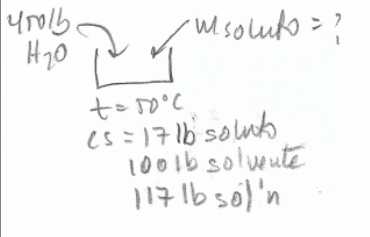
\includegraphics[width=\linewidth, height=2cm]{./problema1_diagrama.png} % Usa todo el ancho disponible en el minipage.
        \caption{Diagrama del \\ problema}
    \end{minipage}
\end{figure}


\textbf{} % Define las variables y fórmulas utilizadas en el problema.
\begin{itemize}
    \item \(\text{m}_\text{soluto}\) = ? % Define la variable para la masa del soluto.
\end{itemize}

\begin{flalign*}
    \text{m}_\text{H$_2$O} &= 450 \text{ lb} && \\ % Masa de agua destilada.
    T &= 50^\circ\text{C} && \\ % Temperatura.
    \text{CS} &= 17 \text{ lb soluto} && \\ % Concentración de saturación.
    &= 100 \text{ lb solvente} && \\ % Masa total de la solución saturada.
    &= 117 \text{ lb sol'n} &&
\end{flalign*}

\columnbreak % Indica el cambio a la columna derecha.

\noindent\textbf{} % Define el título para la columna derecha.

\textbf{Resolución:} % Define la sección para los incisos y la resolución del problema.

\begin{flalign*}
    \text{m}_\text{soluto} &= 450 \text{ lb H}_2\text{O} \cdot \frac{17 \text{ lb soluto}}{100 \text{ lb H}_2\text{O}} \\ % Calcula la masa de K$_2$SO$_4$.
    &= 246.50 \text{ lb soluto} \\\\ % Resultado de la masa de K$_2$SO$_4$.
    \text{m}_\text{solución} &= 246.50 \text{ lb soluto} + 450 \text{ lb solvente} \\ % Calcula la masa total de la solución saturada.
    &= 696.50 \text{ lb de solución saturada} % Resultado de la masa total de la solución.
\end{flalign*}
\end{multicols} % Finaliza la división en dos columnas.



\newpage % Inicia una nueva página.
\section*{Problema 2} % Título del problema, sin numeración de sección.
\textbf{Problema:}
Determina la masa de cristales de NaNO$_3$ obtenidos cuando 600 lb de solución al 55\% masa de la sal a la temperatura de 60°C se enfrían hasta 10°C (CS = 80), sin que exista pérdida de agua durante el enfriamiento.
\begin{multicols}{2} % Divide el contenido en dos columnas.
\noindent\textbf{} % Define el título para la columna izquierda.

\textbf{Datos:} % Define una sección de datos en la columna izquierda.

\begin{figure}[H]
    \begin{minipage}[t]{0.3\textwidth} % Define un espacio del 30% del ancho del texto.
        \raggedright % Alinea a la izquierda dentro del minipage.
        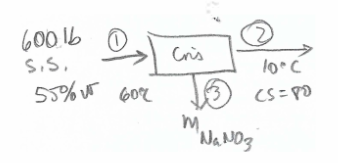
\includegraphics[width=\linewidth, height=2cm]{./problema2_diagrama.png} % Usa todo el ancho disponible en el minipage.
        \caption{Diagrama del \\ problema}
    \end{minipage}
\end{figure}

\textbf{} % Define las variables y fórmulas utilizadas en el problema.
\begin{itemize}
\item m$_1$ = 600 lb (solución inicial)
\item 55\% masa 
\item T$_1$ = 60°C, T$_2$ = 10°C
\item CS = 80
\item m$_3$ = ? (masa de cristales)
\end{itemize}

\columnbreak % Indica el cambio a la columna derecha.

\noindent\textbf{} % Define el título para la columna derecha.

\textbf{Resolución:} % Define la sección para los incisos y la resolución del problema.
\textbf{B. componentes:}

\begin{align*}
    \text{Balance general:} & \quad m_1 = m_2 + m_3 \quad \Rightarrow \quad 600 = m_2 + m_3 \\[10pt]
    \text{Soluto:} & \quad 600 \text{ lb} \times \frac{55 \text{ lb soluto}}{100 \text{ lb soln}} = m_2 \times \frac{80 \text{ lb soluto}}{180 \text{ lb soln}} + m_3 \\[10pt]
    & \quad 330 \text{ lb} = 0.444 \, m_2 + m_3 \\[10pt]
    \text{Solvente:} & \quad 600 \text{ lb} \times \frac{45 \text{ lb solvente}}{100 \text{ lb soln}} = m_2 \times \frac{100 \text{ lb solvente}}{180 \text{ lb soln}} \\[10pt]
    & \quad 270 \text{ lb} = 0.556 \, m_2 \\[10pt]
    m_2 &= \frac{270}{0.556} = 485.61 \text{ lb} \\[10pt]
    m_3 &= 600 - m_2 = 600 - 485.61 = 114.39 \text{ lb cristales}
\end{align*}
\end{multicols} % Finaliza la división en dos columnas.


\newpage % Inicia una nueva página.
\section*{Problema 3} % Título del problema, sin numeración de sección.
\textbf{Problema:} Calcula las masas de solución remanente y de cristales de KBr que se pueden obtener a 30°C (CS = 70), cuando a 15 ton de solución saturada de la sal se le evapora el 35\% del agua presente en la solución, manteniendo la temperatura constante.


\begin{multicols}{2} % Divide el contenido en dos columnas.
\noindent\textbf{Datos:} % Define la sección de datos en la columna izquierda.

\begin{figure}[H]
    \begin{minipage}[t]{0.3\textwidth} % Define un espacio del 30% del ancho del texto.
        \raggedright % Alinea a la izquierda dentro del minipage.
        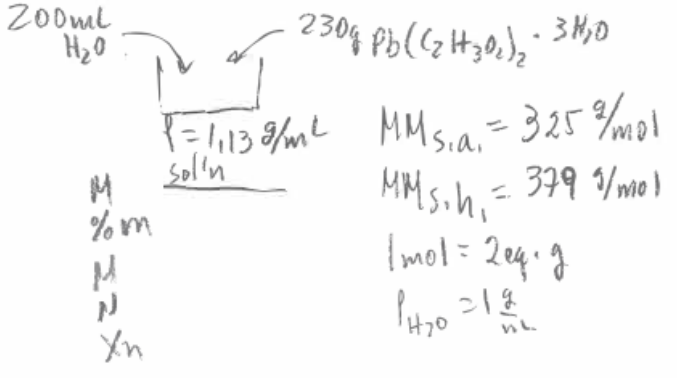
\includegraphics[width=\linewidth, height=2cm]{./problema3_diagrama.png} % Usa todo el ancho disponible en el minipage.
        \caption{Diagrama del \\ problema}
    \end{minipage}
\end{figure}

\textbf{} % Define las variables y fórmulas utilizadas en el problema.
\begin{itemize}
\item m$_1$ = 15 ton (solución inicial)
\item C.S. = 70
\item T$_1$ = 30°C, T$_2$ = 30°C
\item m$_3$ = ? (masa de cristales)
\end{itemize}

\columnbreak % Indica el cambio a la columna derecha.

\noindent\textbf{Resolución:} % Define la sección para los incisos y la resolución del problema.

\textbf{Balance general:}

\begin{align*}
    m_1 &= m_2 + m_3 + m_4 \\[10pt]
    15 &= m_2 + m_3 + m_4 \\[10pt]
    m_4 &= 15 - (m_2 + m_3) \\[10pt]
    m_4 &= 15 - (3.088 + 9.7318) \\[10pt]
    m_4 &= 2.1802 \, \text{ton (solución remanente)}
\end{align*}

\textbf{Balance de componentes:}

\textbf{Soluto:}

\begin{align*}
    x_{m1} &= x_3 m_3 + m_4 \\[10pt]
    15 \, \text{ton} \times \frac{70 \, \text{soluto}}{170 \, \text{soln}} &= \frac{70}{170} m_3 + m_4 \\[10pt]
    6.176 &= 0.412 m_3 + m_4
\end{align*}

\textbf{Solvente:}

\begin{align*}
    y_{1}m_{1} &= \frac{75}{100}y_1 m_1 + \frac{100}{170} m_3 \\[10pt]
    \frac{100}{170} (15 \, \text{ton}) &= 0.35 (8.824) + 0.5882m_3 \\[10pt]
    8.824 - 3.088 &= 0.5882 \, m_3 \\[10pt]
    m_3 &= 9.7318 \, \text{ton (solución remanente)}
\end{align*}

\textbf{Resultado final:}

\begin{align*}
    m_2 &= 3.088 \, \text{ton (agua evaporada)} \\[10pt]
    m_3 &= 9.7318 \, \text{ton (solución remanente)}
\end{align*}
\end{multicols} % Finaliza la división en dos columnas.

\newpage % Inicia una nueva página.
\section*{Problema 4} % Título del problema, sin numeración de sección.
\textbf{Problema:} Se somete a enfriamiento 190 lb de solución saturada de K$_2$SO$_4$ desde 85°C hasta 10°C, perdiéndose durante el proceso 52.3 lb de H$_2$O por evaporación; determina la masa de cristales anhidros que se obtiene.
CS @ 85°C = 22; CS @ 10°C = 10.

\begin{multicols}{2} % Divide el contenido en dos columnas.
\noindent\textbf{Datos:} % Define la sección de datos en la columna izquierda.

\begin{figure}[H]
    \begin{minipage}[t]{0.3\textwidth} % Define un espacio del 30% del ancho del texto.
        \raggedright % Alinea a la izquierda dentro del minipage.
        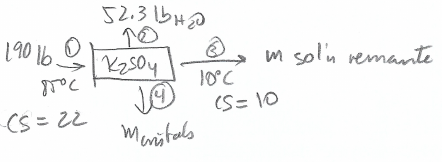
\includegraphics[width=\linewidth, height=2cm]{./problema4_diagrama.png} % Usa todo el ancho disponible en el minipage.
        \caption{Diagrama del \\ problema}
    \end{minipage}
\end{figure}

\textbf{} % Define las variables y fórmulas utilizadas en el problema.
\begin{itemize}
\item m$_1$ = 190 lb (solución inicial)
\item C.S. = 22, C.S. final = 10
\item T$_1$ = 87°C, T$_2$ = 10°C
\item m$_3$ = ? (masa de cristales)
\item m$_4$ = ? (masa de solución remanente)
\end{itemize}

\columnbreak % Indica el cambio a la columna derecha.

\noindent\textbf{Resolución:} % Define la sección para los incisos y la resolución del problema.

\textbf{Balance general:}

\begin{align*}
    m_1 &= m_2 + m_3 + m_4 \\[10pt]
    190 &= 52.3 + m_3 + m_4 \\[10pt]
    137.7 &= m_3 + m_4
\end{align*}

\textbf{Balance de componentes:}

\textbf{Soluto:}

\begin{align*}
    \frac{190 \times 22}{122} &= \frac{10}{110}m_3 + m_4 \\[10pt]
    34.262 &= 0.091 m_3 + m_4
\end{align*}

\textbf{Solvente:}

\begin{align*}
    \frac{190 \times 100}{122} &= 52.3 + \frac{100}{110} m_3 \\[10pt]
    155.738 &= 52.3 + 0.909 m_3 \\[10pt]
    m_3 &= \frac{155.738 - 52.3}{0.909} \\[10pt]
    m_3 &= 113.793 \, \text{lb (cristales)}
\end{align*}

\textbf{Resultado final:}

\begin{align*}
    m_4 &= 137.7 - m_3 \\[10pt]
    m_4 &= 137.7 - 113.793 \\[10pt]
    m_4 &= 23.907 \, \text{lb (solución remanente)}
\end{align*}
\end{multicols} % Finaliza la división en dos columnas.


\newpage % Inicia una nueva página.
\section*{Problema 5} % Título del problema, sin numeración de sección.
\textbf{Problema:} En un proceso de cristalización se desea obtener 250 kg de cristales de NaNO$_3$ al enfriar una solución saturada de la sal desde 60°C (CS = 125) hasta 15°C (CS = 84); si durante el proceso se pierden 115 kg de agua, calcula la masa de solución saturada que deberá alimentarse y la masa de solución saturada remanente.

\begin{multicols}{2} % Divide el contenido en dos columnas.
\noindent\textbf{Datos:} % Define la sección de datos en la columna izquierda.

\begin{figure}[H]
    \begin{minipage}[t]{0.3\textwidth} % Define un espacio del 30% del ancho del texto.
        \raggedright % Alinea a la izquierda dentro del minipage.
        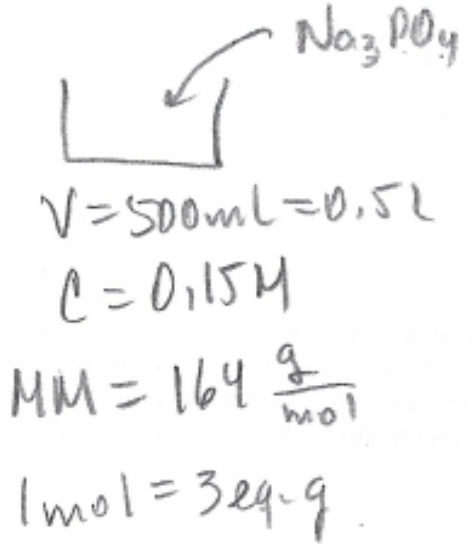
\includegraphics[width=\linewidth, height=2cm]{./problema5_diagrama.png} % Usa todo el ancho disponible en el minipage.
        \caption{Diagrama del \\ problema}
    \end{minipage}
\end{figure}

\textbf{} % Define las variables y fórmulas utilizadas en el problema.
\begin{itemize}
\item m$_1$ = ? (solución inicial)
\item C.S. inicial = 125, C.S. final = 84
\item T$_1$ = 60°C, T$_2$ = 150°C
\item m$_2$ = 115 kg (agua)
\item m$_3$ = ? (solución remanente)
\item m$_4$ = 250 kg (cristales)
\end{itemize}

\columnbreak % Indica el cambio a la columna derecha.

\noindent\textbf{Resolución:} % Define la sección para los incisos y la resolución del problema.

\textbf{Balance general:}

\begin{align*}
    m_1 &= m_2 + m_3 + m_4 \\[10pt]
    m_1 &= 115 + m_3 + 250 \\[10pt]
    m_1 - m_3 &= 365
\end{align*}

\textbf{Balance de componentes:}

\textbf{Soluto:}

\begin{align*}
    \frac{125}{225} m_1 &= \frac{84}{184} m_3 + 250 \\[10pt]
    0.556 m_1 - 0.457 m_3 &= 250
\end{align*}

\textbf{Solvente:}

\begin{align*}
    \frac{100}{225} m_1 &= \frac{100}{184} m_3 + 115 \\[10pt]
    0.444 m_1 - 0.543 m_3 &= 115
\end{align*}

\textbf{Resolviendo simultáneamente:}

\begin{align*}
    m_1 &= 535.938 \, \text{kg (alimentada)} \\[10pt]
    m_3 &= 170.938 \, \text{kg (remanente)}
\end{align*}
\end{multicols} % Finaliza la división en dos columnas.




\end{document} % Finaliza el documento.